\documentclass{article}
\pagestyle{empty}
\usepackage{tikz}
\usetikzlibrary{patterns}
\usetikzlibrary{shapes.geometric}
\usetikzlibrary {shapes.symbols}
\usepackage{pgfplots}
\usepackage{float}
\usepackage{xcolor}
\usepackage[paperwidth=8.7cm,paperheight=5.6cm]{geometry}
\usepackage{pgffor}

%Define my colors
%\definecolor{MyRed}{rgb}{0.95,0.04,0.18}
%\definecolor{MyGreen}{rgb}{0.18,0.95,0.04}
%\definecolor{MyBlue}{rgb}{0.04,0.18,0.95}
\definecolor{MyOrange}{rgb}{0.90,0.48,0.28}
\definecolor{MyViolet}{rgb}{0.63,0.45,0.90}
\definecolor{MyGreen}{rgb}{0.40,0.90,0.66}

%Commands
%Command for the rhomb
\newcommand{\rhomb}[3]{
    \foreach \i in {1,...,#3}{
        \begin{tikzpicture} 
            \node[diamond,draw,minimum height = 3cm, minimum width = 1.5cm,very thick,#1,#2 #1] {};
        \end{tikzpicture}
    }
}

%Command for the not-circle
\newcommand{\NotCircle}[3]{
    \foreach \i in {1,...,#3}{
        \begin{tikzpicture}
            \draw[rounded corners=22,very thick,#1,#2 #1] (-0.75,-1.5) rectangle (0.75,1.5);
        \end{tikzpicture}
    }
}

%Command for the duck shape
\newcommand{\duck}[3]{
    \foreach \i in {1,...,#3}{
        \begin{tikzpicture}
            \node [tape,draw,tape bend top=out and in, tape bend bottom=out and in,minimum height = 1.26cm, minimum width = 3cm,rotate=90,tape bend height = 0.24cm,very thick,#1,#2 #1] {};
        \end{tikzpicture}
    }
}

\begin{document}

\input{TexFile.txt}

\newpage

\begin{figure}[H]
    \centering
    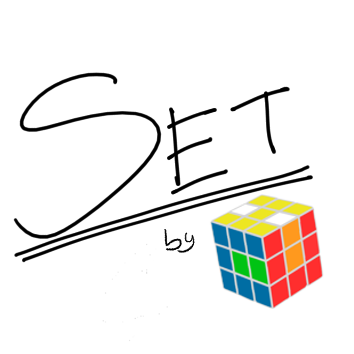
\includegraphics[scale=1.5]{SetLogo.png}
\end{figure}

\newpage

\begin{figure}[H]
    \centering
    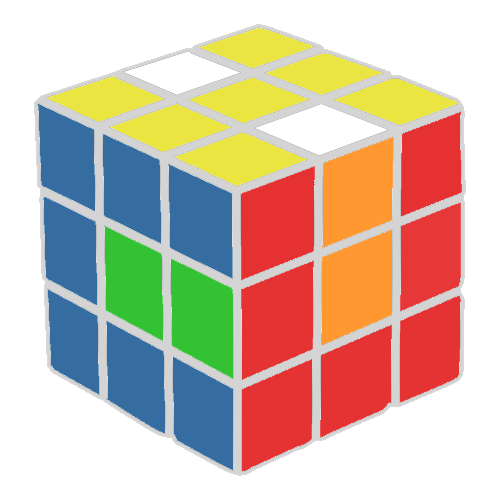
\includegraphics[scale=0.2]{logo2.png}
\end{figure}

\end{document}